\chapter{Chip Summary and Final Conclusions}
	
		The complete circuit design is the final product of this work. It is based on the three previous chapters explaining the design of the chip's individual components. This chapter explains the final layout with connecting pads and lists the final full-chip simulations. The chip is compared to design specifications and potential improvements are discussed. The report is wrapped up with some final conclusions.
		
		%The complete chip-performance has been simulated, both with EM-models of each sub-circuit and for s
		%

	\section{Layout}
		The complete chip is designed to fit into a \unit[4$\times$5]{mm} QFN-package (\autoref{fig:final_chip}). The chip components are placed according to a few requirements:

		First of all, the incoming RF- and outgoing IF-port should ideally be placed on opposite sides of the chip. In order to avoid interference, it would be preferable to have the LO-port on one of the remaining sides. Early on, a straight signal path was favored over more complex choices although this wasn't really a requirement and was relaxed as the chip-layout matured. %The size of the chip had to be \unit[2.4x3.4]{mm} as a smaller

		The diplexer is a big sub-circuit and rather significant to the entire chip-function and at large decides the placement of other circuits on the chip. The LO-amplifier is quite small and connects straight to the mixer. The remaining sub circuits: Two IF-amplifiers and three attenuators are adjusted to fit together.

		The final layout has the RF-port and IF-port on opposite short sides of the chip coupled with ground-pads. No other pads are placed on the short sides to keep the bonding wires isolated. The LO-signal and two bias-signals for the mixer and LO-amplifier respectively are connected on one of the long sides. The bias-signals for the two circuits are separated and isolated with two grounded pads. This gives the possibility of biasing the mixer and/or the amplifier with signals different from \unit[5]{V} in the future.
	
		On the remaining long side, three \unit[5]{V} bias-signals for the IF1-, IF2-amplifiers and the attenuator-circuit enters, as well as three control-signals for the attenuators.
		
		Grounded pads are placed next to the major bias-pads. They are put there in order to make accurate measurements of the naked chip. These pads are however not connected to exterior bonding pads for the packaged chip.

		\begin{figure}[hbt!]
			\centering
			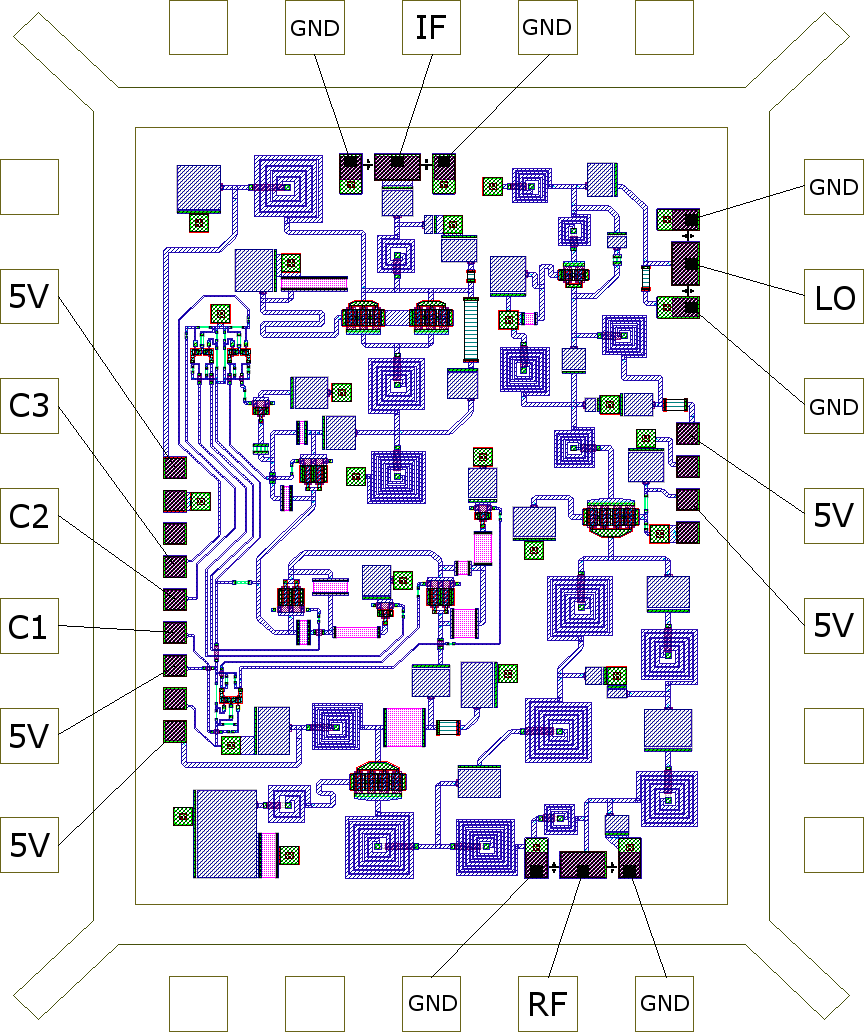
\includegraphics[width=1.0\textwidth]{fig/summary/package}
			\caption[Layout of the pad-structure.]{Layout of the MMIC and labels of the bonding pads. The size of the final package is \unit[4$\times$5]{mm}. The effective chip area containing all components is \unit[2.3$\times$3.3]{mm}. C1, C2 and C3 provide the control signals for the \unit[6]{dB}, \unit[3]{dB} and \unit[1.5]{dB} attenuators respectively.}\label{fig:final_chip}
		\end{figure}

	\section{Performance}
		\subsection{Summary}
			Summary of simulated chip performance at nominal gain (\autoref{tab:chipsummary_nominal}), maximum gain (\autoref{tab:chipsummary_maximum}) and minimum gain (\autoref{tab:chipsummary_minimum}).
			
			\begin{table}[hbt!]
				\caption[Summarized chip performance at nominal gain.]{Summary of chip performance at nominal gain. LO drive at \unit[-2]{dBm}.\disclaimer}
				\label{tab:chipsummary_nominal}
				\centering
				\begin{tabular}{ l c c c c c c l } \toprule
					Parameter & Min. & Typ. & Max. & Min. & Typ. & Max. & Unit \\\midrule
					Frequency range RF & \multicolumn{3}{c}{2.9--3.4} & \multicolumn{3}{c}{3.1--3.3} & GHz \\
					Frequency range LO & \multicolumn{3}{c}{5.04--5.54} & \multicolumn{3}{c}{5.24--5.44} & GHz \\
					Frequency IF & \multicolumn{3}{c}{2.14} & \multicolumn{3}{c}{2.14} & GHz \\
					Return loss RF & 14 & 16 &  & 20 & 21 &  & dB \\
					Return loss LO & 13.5 & 17 &  & 17 & 18 &  & dB \\
					Return loss IF & 23 & 24 &  & 23 & 24 &  & dB \\
					Conversion gain & 10.3 & 10.6 & 10.8 & 10.7 & 10.8 & 10.8 & dB \\
					Gain variation & & 0.45 & 0.45 & & 0.05 & 0.05 & dB \\
					Image rejection & 48 & 50 &  & 50 & 51 &  &  dB \\
					$P_{1dB}$ (input) & 9.8 & 10.0 &  & 9.8 & 10.0 &  & dBm \\
					$IIP_3$ (estimate) & 20 & 20 &  & 20 & 20 &  & dBm \\
					Noise figure (estimate) &  & 11 & 11 &  & 11 & 11 & dB \\
					Power consumption &  & 1.0 & 1.0 &  & 1.0 & 1.0 & W \\\bottomrule
				\end{tabular}
			\end{table}
			
			\begin{table}[hbt!]
				\caption[Summarized chip performance at maximum gain.]{Summary of chip performance at maximum gain (\unit[+4.5]{dB}). Only parameters which performance has changed compared to the case with nominal gain are presented. LO drive at \unit[-2]{dBm}.\disclaimer}
				\label{tab:chipsummary_maximum}
				\centering
				\begin{tabular}{ l c c c c c c l } \toprule
					Parameter & Min. & Typ. & Max. & Min. & Typ. & Max. & Unit \\\midrule
					Frequency range RF & \multicolumn{3}{c}{2.9--3.4} & \multicolumn{3}{c}{3.1--3.3} & GHz \\
					Return loss IF & 29 & 31 &  & 29 & 31 &  & dB \\
					Conversion gain & 14.7 & 15.0 & 15.2 & 15.1 & 15.2 & 15.2 & dB \\
					$P_{1dB}$ (input) & 6.6 & 6.7 &  & 6.6 & 6.7 &  & dBm \\
					$IIP_3$ (estimate) & 17 & 17 &  & 17 & 17 &  & dBm \\
					Noise figure (estimate) &  & 10 & 10 &  & 10 & 10 & dB \\\bottomrule
				\end{tabular}
			\end{table}
			
			\begin{table}[hbt!]
				\caption[Summarized chip performance at minimum gain.]{Summary of chip performance at minimum gain (\unit[-6.0]{dB}). Only parameters which performance has changed compared to the case with nominal gain are presented. LO drive at \unit[-2]{dBm}.\disclaimer}
				\label{tab:chipsummary_minimum}
				\centering
				\begin{tabular}{ l c c c c c c l } \toprule
					Parameter & Min. & Typ. & Max. & Min. & Typ. & Max. & Unit \\\midrule
					Frequency range RF & \multicolumn{3}{c}{2.9--3.4} & \multicolumn{3}{c}{3.1--3.3} & GHz \\
					Return loss IF & 21 & 22 &  & 21 & 22 &  & dB \\
					Conversion gain & 4.3 & 4.6 & 4.8 & 4.7 & 4.8 & 4.8 & dB \\
					$P_{1dB}$ (input) & 11.3 & 11.5 &  & 11.3 & 11.5 &  & dBm \\
					$IIP_3$ (estimate) & 21 & 21 &  & 21 & 21 &  & dBm \\
					Noise figure (estimate) &  & 13 & 13 &  & 13 & 13 & dB \\\bottomrule
				\end{tabular}
			\end{table}
			
		\subsection{Return loss}
			The return losses at the RF- and LO-ports are simulated and found to be very similar as those simulated for the individual components. The results are listed in the chip summary but for detailed frequency characteristics see \autoref{fig:mixermatch} for the RF-port and \autoref{fig:lo_reflections} for the LO-port. The IF-port's return loss depends on the gain setting and is found to be at least \unit[21]{dB} in all cases with a \unit[100]{MHz} bandwidth.
			
		\subsection{Conversion gain}
			The chip's conversion gain is simulated for all gain states in \autoref{fig:sysgainstates} and for different LO drives in \autoref{fig:sysgainvslo}. The IF-signal has a narrow bandwidth. Even so, the \unit[20]{MHz} on the MMIC that it does occupy, exhibits a frequency dependent gain according to \autoref{fig:ifbehave}. This plot is also interesting, should the frequency characteristics in the IF-path shift.
			
			\begin{figure}[hbt!]
				\centering
				\includerect{0.8\textwidth}{fig/summary/gainvsstate}
				\caption[Chip gain for all gain states.]{Chip gain versus frequency for all gain states. $P_{lo}=\unit[-2]{dBm}$. The least significant bit (LSB) is \unit[1.55]{dB} and the dynamic gain is \unit[10.3]{dB}.}\label{fig:sysgainstates}
			\end{figure}
			
			\begin{figure}[hbt!]
				\centering
				\includerect{0.8\textwidth}{fig/summary/gainvslo}
				\caption[Chip gain for different LO drives.]{Chip gain versus frequency for different LO drives at nominal gain. The gain variation is kept below \unit[0.6]{dB} between \unit[2.9 and 3.4]{GHz} for $P_{lo}$=\unit[-4 to 0]{dBm}.}\label{fig:sysgainvslo}
			\end{figure}
			
			\begin{figure}[hbt!]
				\centering
				\includerect{0.8\textwidth}{fig/summary/ifbehave}
				\caption[IF-frequency dependent chip gain.]{IF-frequency dependent chip gain. The gain variation in the \unit[20]{MHz} wide IF band is \unit[0.2]{dB}}\label{fig:ifbehave}
			\end{figure}
			
		\subsection{Linearity}
			Chip $P_{1dB}$ for different gain states and LO drives are plotted in \autoref{fig:sysp1db}. The linearity is as expected highest for minimum gain and lowest for maximum gain. $P_{1dB}$ tends to drop for smaller LO-drives. 
			
%			\begin{figure}[hbt!]
%				\centering
%				\includerect{0.8\textwidth}{fig/summary/chipcompression}
%				\caption[Chip gain compression.]{Chip gain compression at different gain states and for different LO input powers. Traces with $\triangle$ are measured at maximum gain, $\medsquare$ at nominal gain and $\diamond$ at minimum gain. The LO powers range between \unit[-4 and 0]{dBm}. Compression occurs earlier for higher gain. The results are summarized using $P_{1dB}$ in \autoref{fig:sysp1db}.}\label{fig:syscompression}
%			\end{figure}
			
			\begin{figure}[hbt!]
				\centering
				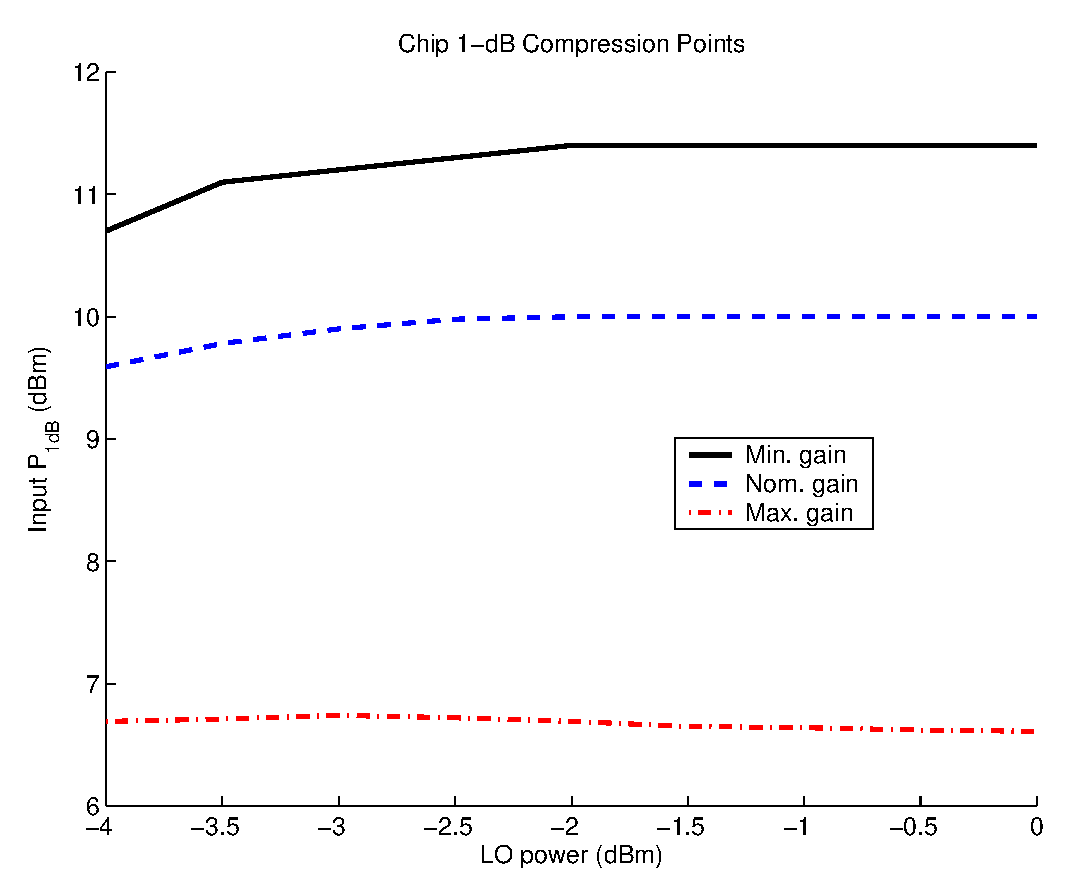
\includegraphics[width=0.8\textwidth]{fig/summary/chipp1db}
				\caption[Chip $P_{1dB}$.]{Chip $P_{1dB}$ for different gain states versus input LO power.}\label{fig:sysp1db}
			\end{figure}
			
		\subsection{Spectrum and spurious frequencies}
			The frequency spectrum from \unit[0 to 10]{GHz} at the output IF port is shown in \autoref{fig:sysspectrum}. The LO isolation is \unit[21]{dB}, which is just above the required level of \unit[20]{dB}. The 2$\times$IF-signal suppression is \unit[38]{dBc}, which is \unit[2]{dB} below the required value. The RF-signal has only \unit[7.6]{dB} isolation.
			
			\begin{figure}[hbt!]
				\centering
				\includerect{1.0\textwidth}{fig/summary/spectrum}
				\caption[IF-port output spectrum.]{Frequency spectrum at the output IF-port for input frequency \unit[3.2]{GHz}, $P_{lo}=\unit[-2]{dBm}$ and nominal gain. Noteworthy components are: IF (\unit[2.14]{GHz}), RF (\unit[3.2]{GHz}), LO (\unit[5.34]{GHz}), 2$\times$IF (\unit[4.28]{GHz}), RF-IF (\unit[1.06]{GHz}) and RF+IF (\unit[8.54]{GHz}). Some of the smaller components are spurious frequencies predicted in \autoref{tab:introsingletone}.}\label{fig:sysspectrum}
			\end{figure}
			

			
		\subsection{Maximum rating}
			All the components are scaled to survive a maximum input power level of $P_{RF}=\unit[17]{dBm}$. This is the maximum power the circuit prior to this mixer chip is able to deliver. The major concerns are the resistors' widths and the width of the microstrips. The sizes are scaled according to UMS specifications.\autocite{pph25manual}
			
			Transistors may not survive if the junction temperature becomes too high. The FETs in the IF-amplifiers run the risk of overheating due to their large current consumption. They are designed to survive a maximum chip backside temperature of \unit[100]{$^\circ$C} which is thought possible in the event of starting the system in a warm dessert for example.
			
	
	\section{Temperature and yield analysis}	
		\subsection{Components}
			Components are affected by temperature as well as production spread. An analysis of the chip performance for different temperatures and yields has been performed. The chip is required to keep its performance between \unit[-40]{$^\circ$C} and \unit[55]{$^\circ$C} and to function up to \unit[85]{$^\circ$C}. 			
			
			The temperature dependence arise mostly in the TiWSi- and GaAs-resistors where the resistance differs $\sim$\unit[10]{\%} as temperature goes from \unit[20]{$^\circ$C} to \unit[85]{$^\circ$C}. The FETs have a temperature dependence as well but the PPH25 models only allow simulations at \unit[20]{$^\circ$C}. Some qualitative arguments can be made by reviewing PH25 FET performance. The gain in PH25 FETs have approximately a \unit[-0.2]{$\%$/K} dependence and this is believed to hold for PPH25 as well considering how similar the processes are. This gives an extra gain of \unit[0.5]{dB} at \unit[-40]{$^\circ$C} and decreases the gain of each FET with \unit[0.25]{dB} at \unit[55]{$^\circ$C}.		

		\subsection{Conversion gain}
			The entire chip's conversion gain is simulated for temperatures between \unit[-40]{$^\circ$C} and \unit[85]{$^\circ$C} (\autoref{tab:chip_temperature_dependence}). The conversion gain increases slightly as temperature increases to \unit[85]{$^\circ$C}. It is believed that the unaccounted temperature dependence of the FET's gain has a reverse effect on the increased chip gain. %Using data from PH25, a FET's gain drops approximately \unit[0.5]{dB} as temperature goes from \unit[20 to 85]{$^\circ$C}. % 60*(-0.2) = -12% gain at 85C. Which gives 10*log(1-60*0.002) = -0.5dB

			
		By taking temperature, yield and the FET's temperature dependence into account, the minimum and maximum chip conversion gain is \unit[9.4]{dB} at \unit[55]{$^\circ$C} and \unit[12]{dB} at \unit[-40]{$^\circ$C}, respectively. This is at the nominal gain state.


		\begin{table}[h!]
				\caption[Chip conversion gain temperature dependence]{Chip conversion gain with yield analysis at nominal gain. The simulation is performed with circuit models where the resistors are adjusted for temperature. PPH25 FET models can only be simulated at \unit[20]{$^\circ$C} and the decreased gain of the FETs at higher temperatures is therefore not included.}
				\label{tab:chip_temperature_dependence}
				\centering
				\begin{tabular}{ l c } \toprule % Circuit simulation gain: 2.6 3.2, 3.5, 3.9
					Temperature & Conversion gain \\\midrule
					\unit[-40]{$^\circ$C} 	& $\unit[10.0\pm1]{dB}$\\
					\unit[20]{$^\circ$C} 	& $\unit[10.6\pm1]{dB}$\\
					\unit[55]{$^\circ$C} 	& $\unit[10.9\pm1]{dB}$ \\
					\unit[85]{$^\circ$C}	& $\unit[11.3\pm1]{dB}$ \\\bottomrule
				\end{tabular}
			\end{table}			
	

		\subsection{Compression point}
		The \unit[1]{dB}-compression point could not be successfully simulated using circuit models and therefore a qualitative argument must be made using performance of sub-circuits and theory.
		
		Since the gain of the FETs decrease with temperature, it can be argued that the IF-amplifiers' compression-points will not decrease at higher temperatures. The LO-amplifier loses \unit[0.4]{dB} of gain at \unit[55]{$^\circ$C} due to its TiWSi-feedback loop and reduced FET-gain which may affect the mixer $P_{1dB}$ with as much. This does not affect the chip compression point by more than \unit[-0.1]{dB} at nominal gain. It is therefore probable that higher temperatures will not affect the chip compression point more than \unit[-0.1]{dB}. 
		
		At temperatures close to \unit[-40]{$^\circ$C}, the gain of each FET increases with \unit[0.5]{dB}. As a side effect, the IF-amplifiers' compression-points decrease with \unit[0.5]{dB} which decreases the chip compression point with \unit[-0.2]{dB} according to the cascade formulas, \autoref{eq:casciip3}. The positive effect of having a larger LO drive is unaccounted for.	This analytical approach results in the chip's compression point being rather temperature-invariant. The yield analysis shows a smallest mixer $P_{1dB}$ of \unit[10]{dB} at $P_{lo}=\unit[-4]{dBm}$. With a \unit[0.5]{dB} and \unit[0.5]{dB} decrease in $P_{1dB}$ for the IF-amplifiers respectively, the effect on the chip's \unit[1]{dB}-compression point is a decrease of \unit[1]{dB} at nominal gain.
		
		By using the yield analysis of sub-circuits and an analytical temperature analysis, the chip $P_{1dB}$ is believed to lose \unit[$\sim$1]{dB} at \unit[-40]{$^\circ$C}.

	
	\section{Discussion}
		\subsection{Comparison to design specifications}
			In Tables \ref{tab:syscomparisonnarrow} and \ref{tab:syscomparisonbroad} is a comparison between design specifications and the simulated chip performance shown. The nominal gain is approximately \unit[1]{dB} higher than specified. This is acceptable, considering that the dynamic gain range is \unit[10.5]{dB} and that the gain empirically is lower than simulated.
			
%			\ctable[ caption = Achieved performance compared to design specifications. For many parameters there is no target specification and the entry is left blank. As chip performance varies a lot with choice of frequency band the comparisons are made for both bands separately. The performance of parameters that don't meet the requirements are stated in the table. Some explanations and exceptions are listed at the bottom.,
%				label = tab:syscomparison,
%				pos = hbt! ]
%				{ l l l l l }
%				{
%  				 \tnote[*]{Chip conversion gain.}
%			 	 \tnote[$\dagger$]{\unit[13]{dB} at minimum gain.}
%				 \tnote[$\ddagger$]{\unit[13]{dB} at input power \unit[-4]{dBm}.}
%				 \tnote[$\S$]{\unit[10]{dB} at input power \unit[-4]{dBm}.}
%				 \tnote[||]{2$\times$IF at \unit[4.28]{GHz}.}}
%				{
%					\multirow{2}{*}{Parameters} & \multicolumn{2}{c}{\unit[3.1--3.3]{GHz}} & \multicolumn{2}{c}{\unit[2.9--3.4]{GHz}} \\
%					& Required & Target & Required & Target \\\hline
%					Temp. function\tmark[*] & Ok &  & Ok &  \\
%					Temp. performance\tmark[*] & Ok &  & Ok &  \\
%					LO input power & \unit[-4--0]{dBm} & &  \unit[-4--0]{dBm} & \\
%					Nominal gain & Ok & & Ok & \\
%					Gain variation & Ok & & Ok & \\
%					Gain control & Ok & & Ok & \\
%					Noise figure & Ok & Ok\tmark[$\dagger$] & Ok & Ok\tmark[$\dagger$] \\
%					Return loss RF & Ok & & \unit[13.5]{dB} & \\
%					Return loss IF & Ok & & Ok & \\
%					Return loss LO & Ok\tmark[$\ddagger$] & & \unit[13]{dB}\tmark[$\S$] & \\
%					$IIP_3$ & Ok & Ok & Ok & Ok \\
%					LO to IF isolation & Ok & & Ok & \\
%					Image rejection & Ok & & Ok & \\
%					RF+LO suppression & Ok & & Ok & \\
%					Other mixing spurs & \unit[-38]{dBc}\tmark[||] & & \unit[-38]{dBc}\tmark[||] & \\
%					Max input power RF & Ok	& & Ok & \\
%					Bias \unit[+5]{V} & Ok & & Ok & \\
%					Power consumption & Ok & Ok & Ok & Ok \\
%					Control signals & Ok & & Ok & \\
%					Package & Ok \unit[4$\times$5]{mm} & & Ok \unit[4$\times$5]{mm} & \\\hline
%				}

			\ctable[ caption = Achieved performance compared to design specifications for frequencies 3.1--3.3 GHz. For many parameters there is no target specification and the entry is left blank. Explanations and exceptions are listed at the bottom.,
				mincapwidth = 1.0\textwidth,
				label = tab:syscomparisonnarrow,
				pos = hbt! ]
			{ l l l l l }
			{
			 \tnote[*]{For nominal gain. $\nf=\unit[13]{dB}$ at minimum gain.}
		 	 \tnote[$\dagger$]{For $P_{LO}$=\unit[-4--0]{dBm}.}
			 \tnote[$\ddagger$]{For nominal gain. $IIP_3=\unit[17]{dB}$ at maximum gain.}
			 \tnote[$\S$]{2$\times$IF at \unit[4.28]{GHz}.}%\tnote[||]{2$\times$IF at \unit[4.28]{GHz}.}
			}
			{	\toprule
				& \multicolumn{2}{c}{Specification} & & \\\cmidrule{2-3}
				Parameter & Required & Target & Result & \\\cmidrule{1-4}
				Temp. function & \unit[-40--+85]{$^\circ$C} &  & \unit[-40--+85]{$^\circ$C} & $\surd$ \\
				Temp. performance & \unit[-40--+55]{$^\circ$C} &  & \unit[-40--+55]{$^\circ$C} & $\surd$ \\
				LO input power & \unit[-5--0]{dBm} & &  \unit[-4--0]{dBm} & -- \\
				Nominal gain & \unit[8--10]{dB} & & \unit[10.5]{dB} & $\surd$ \\
				Gain variation & $\le \unit[0.6]{dB}$ & & \unit[0.05]{dB} & $\surd$ \\
				Gain control & $\ge \unit[\pm 5]{dB}$ & & \unit[-6.0 to +4.5]{dB} & $\surd$ \\
				Noise figure & $\le \unit[15]{dB}$ & $\le \unit[12]{dB}$ & \unit[11]{dB}\tmark[*] & $\surd$ \\
				Return loss RF & $\ge \unit[15]{dB}$ & & \unit[21]{dB} & $\surd$ \\
				Return loss IF & $\ge \unit[15]{dB}$ & & \unit[24]{dB} & $\surd$ \\
				Return loss LO & $\ge \unit[15]{dB}$ & & \unit[14]{dB}\tmark[$\dagger$] & -- \\
				$IIP_3$ & $\ge \unit[15]{dBm}$ & $\ge \unit[17]{dBm}$ & \unit[20]{dBm}\tmark[$\ddagger$] & $\surd$ \\
				LO to IF isolation & >\unit[20]{dB} & & \unit[21]{dB} & $\surd$ \\
				Image rejection & >\unit[30]{dBc} & & \unit[40]{dBc} & $\surd$ \\
				RF+LO suppression & >\unit[40]{dBc} & & \unit[90]{dBc} & $\surd$ \\
				Other mixing spurs & >\unit[40]{dBc} & & \unit[38]{dBc}\tmark[$\S$] & -- \\
				Max input power RF & \unit[17]{dBm} & & \unit[17]{dBm} & $\surd$ \\
				Bias & \unit[+5]{V} & & \unit[+5]{V} & $\surd$ \\
				Power consumption & <\unit[1.5]{W} & <\unit[1.0]{W} & \unit[1.0]{W} & $\surd$ \\
				Control signals & \unit[2.5--3.3]{V} & & \unit[2.5--3.3]{V} & $\surd$ \\
				\multirow{2}{*}{Package} & 4$\times$4, 4$\times$5 & & \multirow{2}{*}{\unit[4$\times$5]{mm}} & \multirow{2}{*}{$\surd$} \\
				&  or \unit[5$\times$5]{mm} &  &  & \\\bottomrule
			}
			
			\ctable[ caption = Achieved performance compared to design specifications. Parameters listed have different result for frequencies 2.9--3.4 GHz compared to the narrower band 3.1--3.3 GHz. The others are listed in \autoref{tab:syscomparisonnarrow}.,
				mincapwidth = 1.0\textwidth,
				label = tab:syscomparisonbroad,
				pos = hbt! ]
			{ l l l l l }
			{
			 %\tnote[*]{For nominal gain. $\nf=\unit[13]{dB}$ at minimum gain.}
		 	 \tnote[*]{For $P_{LO}$=\unit[-4--0]{dBm}.}
			 %\tnote[$\ddagger$]{For nominal gain. $IIP_3=\unit[17]{dB}$ at maximum gain.}
			 %\tnote[$\S$]{2$\times$IF at \unit[4.28]{GHz}.}%\tnote[||]{2$\times$IF at \unit[4.28]{GHz}.}
			}
			{	\toprule
				& \multicolumn{2}{c}{Specification} & & \\\cmidrule{2-3}
				Parameter & Required & Target & Result & \\\cmidrule{1-4}
				LO input power & \unit[-5--0]{dBm} & &  \unit[-4--0]{dBm} & -- \\
				Gain variation & $\le \unit[0.6]{dB}$ & & \unit[0.6]{dB} & $\surd$ \\
				Return loss RF & $\ge \unit[15]{dB}$ & & \unit[16]{dB} & $\surd$ \\
				Return loss LO & $\ge \unit[15]{dB}$ & & \unit[10]{dB}\tmark[*] & -- \\\bottomrule
			}
		
		\subsection{Linearity}
			The chip linearity at nominal gain is measured to $P_{1dB}=\unit[9.8]{dBm}$ with the RF-signal at \unit[3.2]{GHz}. This frequency, the center frequency, has the lowest conversion loss and noise and therefore also the lowest $P_{1dB}$ (as shown in \autoref{fig:mixerp1db}). Using the estimate that $IIP_3=P_{1dB}+\unit[10]{dBm}$ the final $IIP_3$ becomes approximately \unit[20]{dBm}. This is far above the target set at \unit[17]{dBm}.
			
			The high $P_{1dB}$ is needed to provide linear operation even when there is little or no attenuation in the gain block. In the worst case (maximum chip gain) $P_{1dB}$ becomes \unit[6.6]{dBm}. Using the same estimate, $IIP_3$ turns out to be slightly less than \unit[17]{dBm}.
			
			Furthermore, the full chip simulations resulted in a $P_{1dB}$ \unit[2]{dBm} higher than the one calculated using the results from the individual components. This discrepancy is explained by the dynamics of the entire chip working together. Spurious and harmonic frequencies earlier only simulated in the mixer component are now present everywhere. Also, if there is a mismatch between two components this loss will increase $P_{1dB}$. This will unfortunately also increase the noise figure.
			
			The simulation software cannot provide high enough accuracy needed to perform the three-tone simulation ($f_{RF1}$, $f_{RF2}$ and $f_{LO}$) necessary for $IIP_3$, why estimates from $P_{1dB}$-simulations are used instead. Some full-chip, low accuracy $IIP_3$ simulations are however made for reference and they show a $\sim$\unit[3]{dBm} better result than the estimates using $P_{1dB}$. Due to their uncertainty, these results are not listed above. It is interesting to see which results the manufactured chip will adhere to.
			
		\subsection{Noise}
			As PPH25 noise models are unavailable, the noise figures for the individual components are estimated using various methods. The reliability of these noise figures is quite high. Contrary to measuring $P_{1dB}$ on the full chip, noise cannot be simulated but must instead be calculated using a formula similar to the one used for $IIP_3$ (\autoref{sec:casc_iip3}). Calculating $IIP_3$ this way gives a \unit[2]{dB} discrepancy from the complete chip simulation. There is a possibility that this discrepancy in present also in the case of the noise. It is therefore hard to say if the final noise figure result is as reliable as the individual components'.
			
	\section{Conclusions}
		\subsection{Achievements}
			The simulations show that the chip performs well when comparing performance to the specifications. Except for some input matching and input power issues at the LO port all required and targeted goals are met. Chip $IIP_3$ is \unit[3]{dB} above the targeted performance and the noise figure $\nf$ is \unit[1]{dB} below the target.
						
		\subsection{Possible improvements}
			RF-to-IF isolation in the chip is rather weak, only \unit[7.6]{dB} at nominal gain. There is no required level of isolation specified but a RF-signal at the output only \unit[18]{dB} lower than the IF-signal can be considered large. In order to increase the isolation the filtering structure after the mixing FET has to be improved. Components part of this structure are the low-pass filter in the diplexer and the two IF-amplifiers. This is not an easy task as the RF lies close to the IF in frequency. The isolation would be even worse if the first IF amplifier would have wider bandwidth and thus higher gain at the RF frequency (which is possible with parallel feedback).
			
			The high linearity can be traded for lower DC power consumption, if such an interest exists. The present DC power consumption is just below the target of \unit[1.0]{W}. The final IF-amplifier is the part consuming most power in order to achieve high linearity. Decreasing $i_{ds}$ and thereby the power consumption for this amplifier will reduce overall chip $IIP_3$. Since the $IIP_3$ is as high as it is, it might therefore be interesting to cut back on the power.
